Peter hace una bandera de $X$ (marca el lugar) para la búsqueda de un tesoro.
La bandera de tela blanca es cuadrada y sus lados son de 12 centímetros.
Para hacer la $X$ pone el listón diagonalmente de una esquina a otra.

\textbf{¿Cuántos centímetros de listón va a necesitar Peter para hacer la $X$?}\\
\textit{Redondea tu respuesta al centímetro más cercano.}

\begin{solutionbox}{15cm}
    La longitud del listón es la hipotenusa de un triángulo rectángulo.
    \begin{figure}[H]
        \centering
        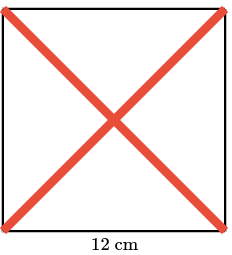
\includegraphics[width=0.2\linewidth]{../images/proverb_pitagoras_10.png}
        \caption{}
        \label{fig:proverb_pitagoras_10}
    \end{figure}
    Podemos usar el teorema de Pitágoras para obtener $x$.
    La ecuación del teorema de Pitágoras es:
    \[c^2=a^2+b^2\]
    donde $a$ y $b$ son las longitudes de los dos catetos del triángulo y $c$ es la longitud de la hipotenusa.
    En este caso, $a=12$, $b=12$ y $c=x$.
    \begin{align*}
        x^2 & =12^2+12^2  \\
        x^2 & =288        \\
        x   & =\sqrt{288} \\
        x   & \sim 16.97
    \end{align*}
    Se necesitarán 17 centímetros de listón para cada línea diagonal. Para obtener la cantidad total de listón necesario, multiplicamos.
    \[17\cdot 2=34\]
    Peter necesitará aproximadamente 34 centímetros de listón para hacer la $X$.
\end{solutionbox}